\documentclass[letter,twoside,11pt]{article}

\usepackage[spanish,es-nodecimaldot]{babel}
\usepackage[utf8]{inputenc}

\usepackage{lmodern}
\usepackage[T1]{fontenc}
\usepackage{textcomp}

\usepackage{framed}
\usepackage[svgnames]{xcolor}
\colorlet{shadecolor}{Gainsboro!50}

\usepackage[labelfont=bf]{caption}
\usepackage{graphicx}
\usepackage{pstricks}

\usepackage{anysize}
\marginsize{3cm}{2cm}{2cm}{3cm}

\usepackage{siunitx}
\usepackage{amsmath}
\usepackage{array}
\usepackage{alltt}
\usepackage{csquotes}

\usepackage{fancyhdr}
\usepackage{lastpage}
\pagestyle{fancy}
\fancyhf{}
\fancyhead[LE,RO]{Electrónica Analógica I}
\fancyfoot[CO,CE]{\thepage\ de \pageref{LastPage}}

\special{papersize=215.9mm,279.4mm}

\usepackage[
    pdfauthor={Carlos Eduardo Caballero Burgoa},%
    pdftitle={Electrónica Analógica I},%
    pdfsubject={Calculo de transistor},%
    colorlinks,%
    citecolor=black,%
    filecolor=black,%
    linkcolor=black,%
    urlcolor=black,
    breaklinks]{hyperref}
\usepackage{breakurl}

\newcommand{\blankpage}{
\newpage
\thispagestyle{empty}
\mbox{}
\newpage
}

\renewcommand{\arraystretch}{1.2}

\DeclareUnicodeCharacter{03A9}{~}

\begin{document}

\begin{titlepage}
    \begin{center}
        {\Large UNIVERSIDAD MAYOR DE SAN SIMÓN}\\
        \vspace*{0.15cm}
        {\large FACULTAD DE CIENCIAS Y TECNOLOGÍA}\\
        \vspace*{0.10cm}
        DEPARTAMENTO DE ELÉCTRICA-ELECTRÓNICA\\
        \vspace*{3.0cm}
        {\Large \textbf{ELECTRÓNICA ANALÓGICA I}}\\
        %\vspace*{0.3cm}
        %{\Large \textbf{REPORTE No. 1}}\\
        \vspace*{3.5cm}
        {\Large \textbf{TRANSISTOR POLARIZADO POR \\ MEDIO DE UN DIVISOR DE VOLTAJE}}\\
    \end{center}

    \vspace*{6.1cm}
    \leftskip=7.95cm
    \noindent
    \textbf{Estudiante:}\\
    Caballero Burgoa, Carlos Eduardo.\\
    Herbas Nava, Adrian.\\
    \newline
    \textbf{Carrera:}\\
    Ing. Electromecánica.\\
    \newline
    \textbf{Docente:}\\
    Ing. Alberto Arispe Santander.\\
    \newline
    \textbf{Grupo:} 2.\\
    \textbf{Fecha de entrega:} 5 de Noviembre del 2024.\\
\end{titlepage}
\addtocounter{page}{-1}

\blankpage
\addtocounter{page}{-1}

Este documento detalla las pruebas que se realizaron sobre un transistor
\textbf{2N2222A} en un divisor de voltaje con una fuente de CD de
$9[\text{V}]$ para cumplir con un conjunto de condiciones definidas, y las
resistencias halladas para una aproximación razonable.

\section{Introducción}
Dado el circuito de la \textbf{figura~\ref{circuito1}} y considerando las
siguientes condiciones:

\begin{equation*}
    \begin{split}
        V_{\text{CC}} &= 9[\text{V}]\\
        V_{\text{CE}} &= \frac{V_{\text{CC}}}{2}\\
        V_{\text{E}} &= 0.1\,V_{\text{CC}}\\
    \end{split}
\end{equation*}

\begin{figure}[!h]
\centering
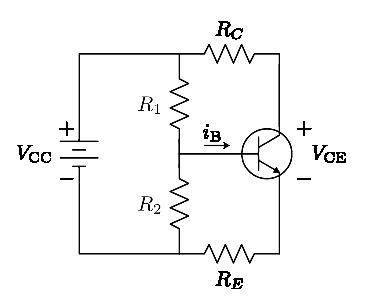
\includegraphics[scale=1.1]{figura1.eps}
\caption{Circuito de polarización con divisor de voltaje.}
\label{circuito1}
\end{figure}

Se hallan los valores de las resistencias que cumplan las condiciones
establecidas.

\section{Análisis exacto}
Para el calculo de los valores del circuito se utiliza el análisis exacto, que
consta de las siguientes ecuaciones \cite{Boylestad}:

\begin{equation*}
    \begin{split}
        R_{\text{TH}} &= \frac{R_1\,R_2}{R_1+R_2}\\
        V_{\text{TH}} &= \frac{R_2}{R_1+R_2}\,V_{\text{CC}}\\
        I_{\text{B}}  &= \frac{V_{\text{TH}}-V_{\text{BE}}}
                         {R_{\text{TH}}+(\beta + 1)\,R_{\text{E}}}\\
        V_{\text{CE}} &= V_{\text{CC}} - I_{\text{C}}\,(R_C + R_E)\\
    \end{split}
\end{equation*}

\section{Hoja de datos 2N2222A}
La hoja de datos del transistor \textbf{2N2222A} se detalla en el
\textbf{Cuadro~\ref{hojadedatos}}.

\begin{table}[!h]
\begin{center}
    \begin{tabular}{|c|l|c|c|c|}
    \hline
    \multicolumn{5}{|c|}{\textbf{Valores nominales absolutos máximos}}
    \tabularnewline \hline
    \textbf{Símbolo} &
    \textbf{Parámetro} &
    \multicolumn{2}{|c|}{\textbf{Valor}} &
    \textbf{Unidades}
    \tabularnewline \hline \hline
    $V_{\text{CEO}}$ &
    Voltaje en colector-emisor &
    \multicolumn{2}{|c|}{$40$} & $V$
    \tabularnewline \hline
    $V_{\text{CBO}}$ &
    Voltaje en colector-base &
    \multicolumn{2}{|c|}{$75$} &
    $V$
    \tabularnewline \hline
    $V_{\text{EBO}}$ &
    Voltaje en emisor-base &
    \multicolumn{2}{|c|}{$6.0$} &
    $V$
    \tabularnewline \hline
    $I_{\text{C}}$ &
    Corriente en el colector &
    \multicolumn{2}{|c|}{$600$} &
    $mA$
    \tabularnewline \hline
    $P_{\text{D}}$ &
    Disipación total del dispositivo &
    \multicolumn{2}{|c|}{$625$} &
    $mW$
    \tabularnewline \hline
    \multicolumn{5}{|c|}{\textbf{Características eléctricas (apagado)}}
    \tabularnewline \hline
    \textbf{Símbolo} &
    \textbf{Parámetro} &
    \textbf{Mín.} &
    \textbf{Máx.} &
    \textbf{Unidades}
    \tabularnewline \hline \hline
    $V_{\text{BR(CEO)}}$ &
    Voltaje de ruptura en colector-emisor &
    $40$ &
    $-$ &
    $V$
    \tabularnewline \hline
    $V_{\text{BR(CBO)}}$ &
    Voltaje de ruptura en colector-base &
    $75$ &
    $-$ &
    $V$
    \tabularnewline \hline
    $V_{\text{BR(EBO)}}$ &
    Voltaje de ruptura en emisor-base &
    $6.0$ &
    $-$ &
    $V$
    \tabularnewline \hline
    $I_{\text{CEX}}$ &
    Corriente de corte en el colector &
    $-$ &
    $10$ &
    $nA$
    \tabularnewline \hline
    $I_{\text{CBO}}$ &
    Corriente de corte en la base &
    $-$ &
    $10$ &
    $nA$
    \tabularnewline \hline
    $I_{\text{EBO}}$ &
    Corriente de corte en el emisor &
    $-$ &
    $10$ &
    $nA$
    \tabularnewline \hline
    \multicolumn{5}{|c|}{\textbf{Características eléctricas (encendido)}}
    \tabularnewline \hline
    \textbf{Símbolo} &
    \textbf{Parámetro} &
    \textbf{Mín.} &
    \textbf{Máx.} &
    \textbf{Unidades}
    \tabularnewline \hline \hline
    $h_{\text{FE}}$ &
    Ganancia de corriente en CD & & & $-$
    \tabularnewline
    & $I_C = 0.1mA,\,V_{\text{CE}} = 10V$ &  $35$ &   $-$ & \tabularnewline
    & $I_C = 1.0mA,\,V_{\text{CE}} = 10V$ &  $50$ &   $-$ & \tabularnewline
    & $I_C =  10mA,\,V_{\text{CE}} = 10V$ &  $75$ &   $-$ & \tabularnewline
    & $I_C = 150mA,\,V_{\text{CE}} = 10V$ & $100$ & $300$ & \tabularnewline
    & $I_C = 500mA,\,V_{\text{CE}} = 10V$ &  $40$ &   $-$ &
    \tabularnewline \hline
    $V_{\text{CE(sat)}}$ &
    Voltaje de saturación en colector-emisor & & & $V$
    \tabularnewline
    & $I_C = 150mA,\,I_B = 15mA$ & $-$ & $0.3$ & \tabularnewline
    & $I_C = 500mA,\,I_B = 50mA$ & $-$ & $1.0$ &
    \tabularnewline \hline
    $V_{\text{BE(sat)}}$ &
    Voltaje de saturación en base-emisor & & & $V$
    \tabularnewline
    & $I_C = 150mA,\,I_B = 15mA$ & $-$ & $1.2$ & \tabularnewline
    & $I_C = 500mA,\,I_B = 50mA$ & $-$ & $2.0$ &
    \tabularnewline \hline
    \end{tabular}
\end{center}
\caption{Hoja de datos parcial 2N2222A.}
\label{hojadedatos}
\end{table}

\section{Resistencias disponibles}
Se cuenta con una seria de resistencias de $0.5[\text{W}]$ con los valores
detallados en el \textbf{Cuadro~\ref{resistencias}}.

\begin{table}
\begin{center}
    \begin{tabular}{|c|c|c|c|c|c|c|c|c|c|}
    \hline
    $1[\Omega]$ & $10[\Omega]$ & $22[\Omega]$ & $47[\Omega]$ & $100[\Omega]$ &
    $150[\Omega]$ & $200[\Omega]$ & $220[\Omega]$ & $270[\Omega]$ &
    $330[\Omega]$
    \tabularnewline \hline
    $470[\Omega]$ & $510[\Omega]$ & $680[\Omega]$ & $1[k{\Omega}]$ &
    $2[k{\Omega}]$ & $2.2[k{\Omega}]$ & $3.3[k{\Omega}]$ & $4.7[k{\Omega}]$ &
    $5.1[k{\Omega}]$ & $6.8[k{\Omega}]$
    \tabularnewline \hline
    $10[k{\Omega}]$ & $20[k{\Omega}]$ & $47[k{\Omega}]$ & $51[k{\Omega}]$ &
    $68[k{\Omega}]$ & $100[k{\Omega}]$ & $220[k{\Omega}]$ & $330[k{\Omega}]$ &
    $510[k{\Omega}]$ & $1[M{\Omega}]$
    \tabularnewline \hline
    \end{tabular}
\end{center}
\caption{Resistencias disponibles para el calculo.}
\label{resistencias}
\end{table}

\section{Calculo de las resistencias}
Haciendo uso del software \emph{Octave} se calculan los valores de resistencias
que combinadas cumplen las condiciones establecidas, con el siguiente programa:

\footnotesize
\begin{shaded}
\begin{verbatim}
% polarizacion por divisor de voltaje
Vcc = 9;            % [V]
Vce = Vcc / 2;      % [V]
Ve = 0.1 * Vcc;     % [V]

Vbe = 0.672;        % [V]

B = 267;

% resistencias disponibles
R = [
    1 ...
    10 22 47 ...
    100 150 200 220 270 330 470 510 680 ...
    1000 2000 2200 3300 4700 5100 6800 ...
    10000 20000 47000 51000 68000 ...
    100000 220000 330000 510000 ...
    1000000
];

count = 1;
printf('\tR1[Ω]\tR2[Ω]\tRC[Ω]\tRE[Ω]\t->\tVce[V]\tVe[V]\tIb[µA]\tIc[mA]\tPC[mW]\tPE[mW]\n');

for (h = 1:length(R))
    for (i = 1:length(R))
        for (j = 1:length(R))
            for (k = 1:length(R))
                R1 = R(h);
                R2 = R(i);
                RC = R(j);
                RE = R(k);

                % metodo exacto
                Rth = (R1 * R2) / (R1 + R2);
                Vth = ( R2 / (R1 + R2) ) * Vcc;

                Ib = (Vth - Vbe) / (Rth + ((B + 1) * RE));
                Ic = B * Ib;
                Ie = (B + 1) * Ib;

                _Vce = Vcc - (Ic * (RC + RE));
                _Ve = Ie * RE;

                if(
                    (abs(_Vce - Vce) < 0.2)&&       % 4.3 < Vce < 4.7[V]
                    (abs(_Ve - Ve) < 0.1)&&         % 0.8 < Ve < 1.0[V]
                    (Ic < 600e-3)&&                 % Ic < 600[mA]
                    (Ib > 200e-6)                   % Ib > 200[µA]
                )
                    printf(
                        '%d\t%d\t%d\t%d\t%d\t->\t%.2f\t%.2f\t%.2f\t%.2f\t%.2f\t%.2f\n',
                        count,
                        R(h),                       % R1
                        R(i),                       % R2
                        R(j),                       % RC
                        R(k),                       % RE
                        _Vce,                       % Vce [V]
                        _Ve,                        % Ve [V]
                        Ib * 1e6,                   % Ib [µA]
                        Ic * 1e3,                   % R1 [mA]
                        Ic * Ic * RC * 1e3,         % Pc [mW]
                        _Ve * Ie * 1e3              % Pe [mW]
                    );

                    count++;
                endif
            endfor
        endfor
    endfor
endfor
\end{verbatim}
\end{shaded}
\normalsize

La salida del programa detalla los valores de las cuatro resistencias ($R_1$,
$R_2$, $R_C$, $R_E$), el voltaje de colector-emisor ($V_{\text{CE}}$), el
voltaje de la resistencia emisor ($V_{\text{E}}$), la corriente de base ($I_B$),
la corriente de colector ($I_C$), la potencia en la resistencia colector ($P_C$)
y la potencia en la resistencia emisor ($P_E$):
\footnotesize
\begin{shaded}
\begin{verbatim}
     R1[Ω]  R2[Ω]   RC[Ω]  RE[Ω]    ->    Vce[V]  Ve[V]    Ib[µA]  Ic[mA]    PC[mW]  PE[mW]
1    1000   200     100    22       ->    4.55    0.81     136.57  36.47     132.97  29.47
2    10000  3300    47     10       ->    4.40    0.81     302.46  80.76     306.53  65.71
3    20000  20000   47     10       ->    4.41    0.81     301.89  80.61     305.37  65.46
4    47000  68000   100    22       ->    4.50    0.81     138.03  36.85     135.81  30.10
5    47000  100000  100    22       ->    4.31    0.85     143.93  38.43     147.68  32.73
6    51000  220000  100    22       ->    4.43    0.83     140.26  37.45     140.26  31.09
7    51000  330000  100    22       ->    4.37    0.84     142.27  37.99     144.29  31.98
8    51000  510000  100    22       ->    4.32    0.85     143.70  38.37     147.21  32.63
\end{verbatim}
\end{shaded}
\normalsize

\section{Simulación}
Se utilizó el software \emph{Quite Universal Circuit Simulator.} versión 23.3.1
para simular el circuito, este puede verse en la
\textbf{Figura~\ref{simulacion1}}.

\begin{figure}[!h]
\centering
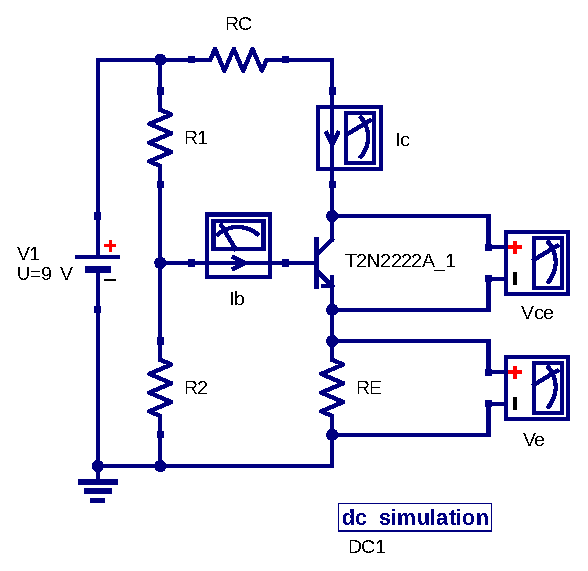
\includegraphics[scale=1.0]{simulacion/npm3.eps}
\caption{Simulación del circuito.}
\label{simulacion1}
\end{figure}

Los valores calculados en el simulador pueden verse en el
\textbf{Cuadro~\ref{simulacion2}}.

\begin{table}[!h]
\begin{center}
    \begin{tabular}{|c|c|c|c||c|c|c|c|}
    \hline
    $R_1[\Omega]$ & $R_2[\Omega]$ & $R_C[\Omega]$ & $R_E[\Omega]$ &
    $V_{\text{CE}}[V]$ & $V_{\text{E}}[V]$ &
    $I_{\text{B}}[\mu{A}]$ & $I_{\text{C}}[mA]$
    \tabularnewline \hline
    $ 1k$ & $ 200$ & $100$ & $22$ & $4.79$ & $0.763$ & $186$ & $34.5$ \tabularnewline \hline
    $10k$ & $3.3k$ & $ 47$ & $10$ & $5.41$ & $0.632$ & $350$ & $62.8$ \tabularnewline \hline
    $20k$ & $ 20k$ & $ 47$ & $10$ & $5.70$ & $0.582$ & $319$ & $57.8$ \tabularnewline \hline
    $47k$ & $ 68k$ & $100$ & $22$ & $5.66$ & $0.605$ & $145$ & $27.4$ \tabularnewline \hline
    $47k$ & $100k$ & $100$ & $22$ & $5.54$ & $0.626$ & $150$ & $28.3$ \tabularnewline \hline
    $51k$ & $220k$ & $100$ & $22$ & $5.65$ & $0.606$ & $145$ & $27.4$ \tabularnewline \hline
    $51k$ & $330k$ & $100$ & $22$ & $5.61$ & $0.613$ & $147$ & $27.7$ \tabularnewline \hline
    $51k$ & $510k$ & $100$ & $22$ & $5.59$ & $0.618$ & $148$ & $28.0$ \tabularnewline \hline
    \end{tabular}
\end{center}
\caption{Valores obtenidos de la simulación.}
\label{simulacion2}
\end{table}

\section{Método experimental}
El circuito armado puede verse en la \textbf{Figura~\ref{armado1}}, alimentado
por una fuente estable de $9[\text{V}]$.

En el circuito se fueron variando las resistencias obtenidas en el calculo
anterior, y se midieron los valores de voltaje y corriente, estos se muestran
en el \textbf{Cuadro~\ref{armado2}}.

\begin{figure}[!h]
\centering
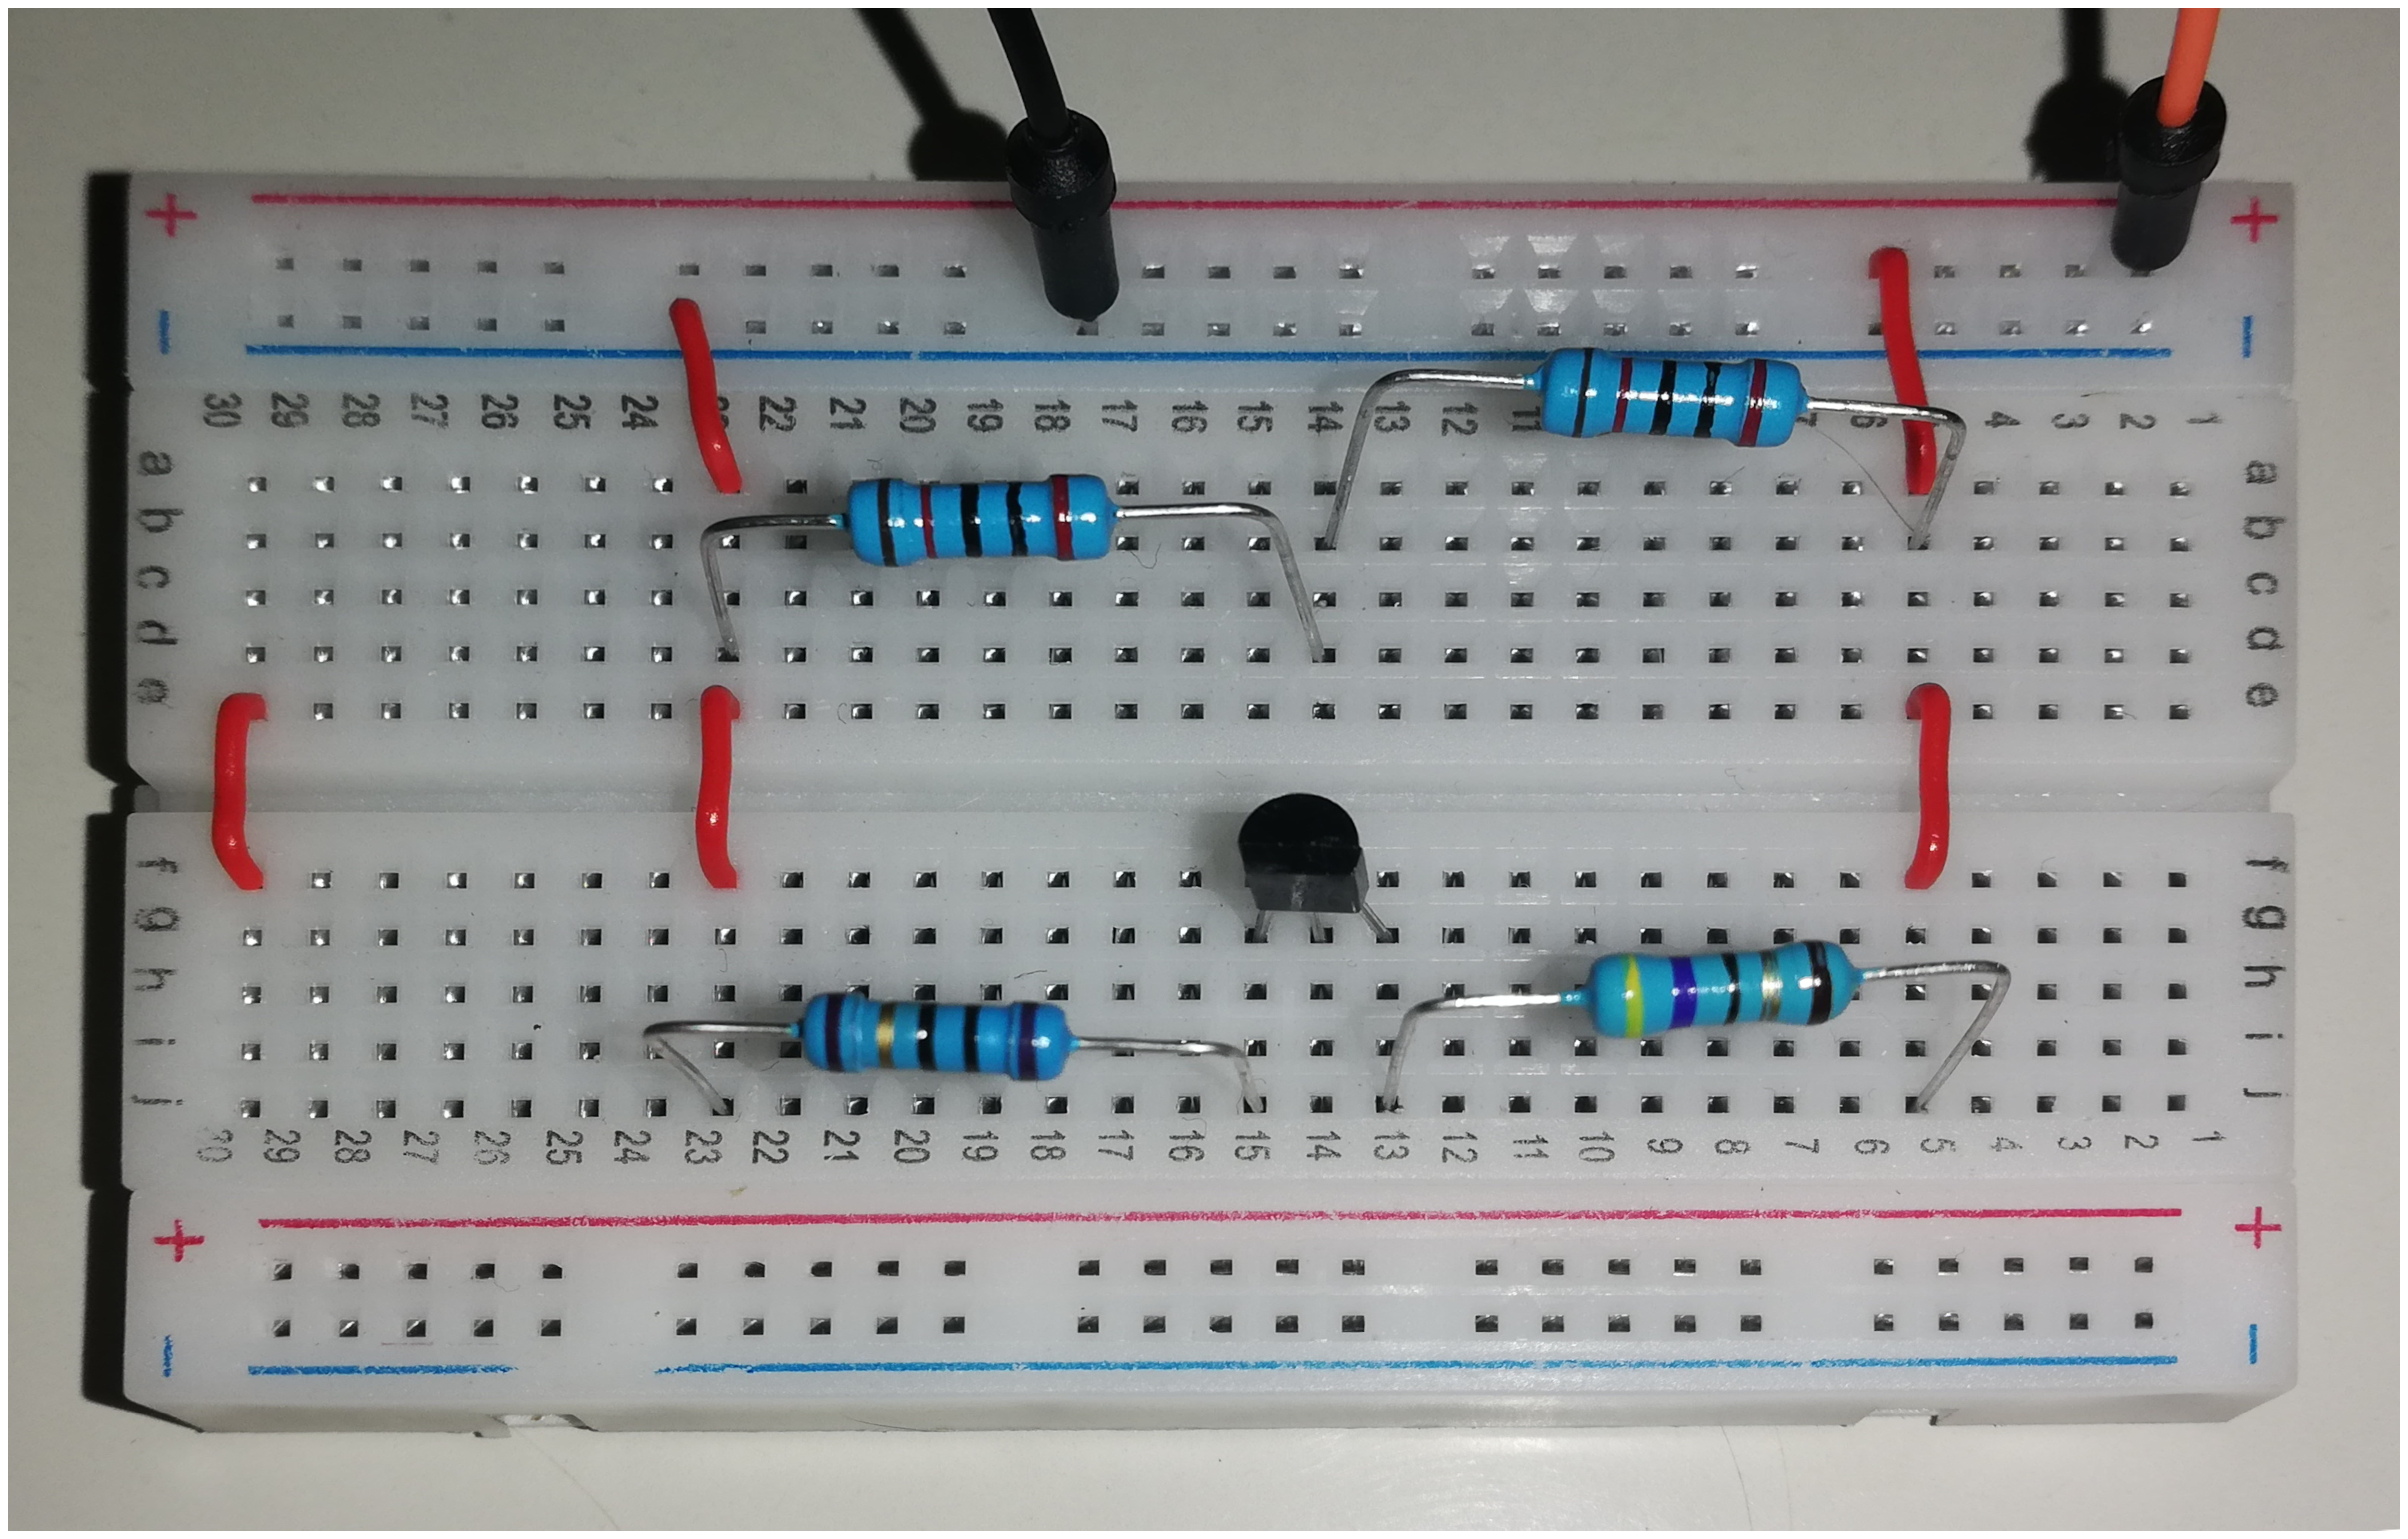
\includegraphics[scale=0.12]{fotos/circuito1.eps}
\caption{Circuito armado.}
\label{armado1}
\end{figure}

\begin{table}[!h]
\begin{center}
    \begin{tabular}{|c|c|c|c||c|c|c|c|}
    \hline
    $R_1[\Omega]$ & $R_2[\Omega]$ & $R_C[\Omega]$ & $R_E[\Omega]$ &
    $V_{\text{CE}}[V]$ & $V_{\text{E}}[V]$ &
    $I_{\text{B}}[\mu{A}]$ & $I_{\text{C}}[mA]$
    \tabularnewline \hline
    $ 1k$ & $ 200$ & $100$ & $22$ & $4.37$ & $0.828$ & $142$ & $37.1$ \tabularnewline \hline
    $10k$ & $3.3k$ & $ 47$ & $10$ & $4.00$ & $0.895$ & $302$ & $87.0$ \tabularnewline \hline
    $20k$ & $ 20k$ & $ 47$ & $10$ & $3.25$ & $1.010$ & $358$ & $95.2$ \tabularnewline \hline
    $47k$ & $ 68k$ & $100$ & $22$ & $4.56$ & $0.823$ & $138$ & $36.1$ \tabularnewline \hline
    $47k$ & $100k$ & $100$ & $22$ & $4.32$ & $0.830$ & $145$ & $36.6$ \tabularnewline \hline
    $51k$ & $220k$ & $100$ & $22$ & $4.42$ & $0.800$ & $141$ & $36.9$ \tabularnewline \hline
    $51k$ & $330k$ & $100$ & $22$ & $4.40$ & $0.831$ & $143$ & $37.0$ \tabularnewline \hline
    $51k$ & $510k$ & $100$ & $22$ & $4.30$ & $0.840$ & $145$ & $36.5$ \tabularnewline \hline
    \end{tabular}
\end{center}
\caption{Valores medidos en la circuito.}
\label{armado2}
\end{table}

\section{Conclusiones y recomendaciones}
Según las pruebas realizadas los valores que mas se aproximan a las condiciones
iniciales son:

\begin{equation*}
    \begin{split}
        R_1 &= 47[k\Omega]\\
        R_2 &= 68[k\Omega]\\
        R_C &= 100[\Omega]\\
        R_E &= 22[\Omega]\\
\end{split}
\end{equation*}

Los valores medidos son muy próximos a los calculados con el programa inclusive
mas que los de la simulación, esto se debe al uso del valor real de voltaje
base-emisor ($V_{\text{BE}}$) y la ganancia del transistor ($h_{\text{FE}}$) en
el calculo.

\begin{thebibliography}{99}

\bibitem{Boylestad}
Boylestad, Robert L. y Nashelsky, Louis. (2009).\\
\textbf{Electrónica: Teoría de Circuitos y Dispositivos Electrónicos. 10ma Edición.}\\
Pearson Educación

\bibitem{2N2222A} 2N2222A Small Signal Switching Transistor\\
Extraído el 3 de Noviembre del 2024, de: \\
\url{https://web.mit.edu/6.101/www/reference/2N2222A.pdf}.

\end{thebibliography}

\end{document}

